\documentclass[./00PhotoBox.tex]{subfiles}
\graphicspath{{\subfix{./img/}}}
\begin{document}


\chapter{Photogrammetrische Grundlagen}
\label{c:photogrammetrie}
Das zu entwickelnde System soll 3D-Modelle von Objekten erstellen. Hierfür wird Photogrammetrie in Form einer \gls{SfM}-Pipeline genutzt.
Der allgemeine Ablauf ist in \autoref{img:ablauf} dargestellt. Zunächst werden die Bilder aufgenommen (siehe \autoref{s:bilder}). Hierbei ist es wichtig, dass die Bildinhalte sich überlappen.
Die Bilder werden dann verknüpft, indem identische Punkte in den Bildern identifiziert werden  (siehe \autoref{s:verknuepfung}). Hierfür können beispielsweise ArUco-Marker oder die SIFT-Methode genutzt werden.
Aus den identifizierten Punkten werden dann die Positionen und Ausrichtung der Kameras und Verknüpfungspunkte in einem lokalen Koordinatensystem ohne bekannten Maßstab berechnet. Die so erzeugten Daten werden anschließend in einer Bündelblockausgleichung gemeinsam optimiert (siehe \autoref{s:buendelblock}). Durch die Nutzung von bekannten Größen, beispielsweise kalibrierte Maßstäbe, kann dieses System transformiert werden, sodass die Größen der Objekte bestimmt werden können.

Dieses Kapitel beschreibt die hierfür notwendigen Bedingungen und die Grundlagen der Rekonstruktion des Objektes als 3D-Modell.

\begin{figure}
    \centering
    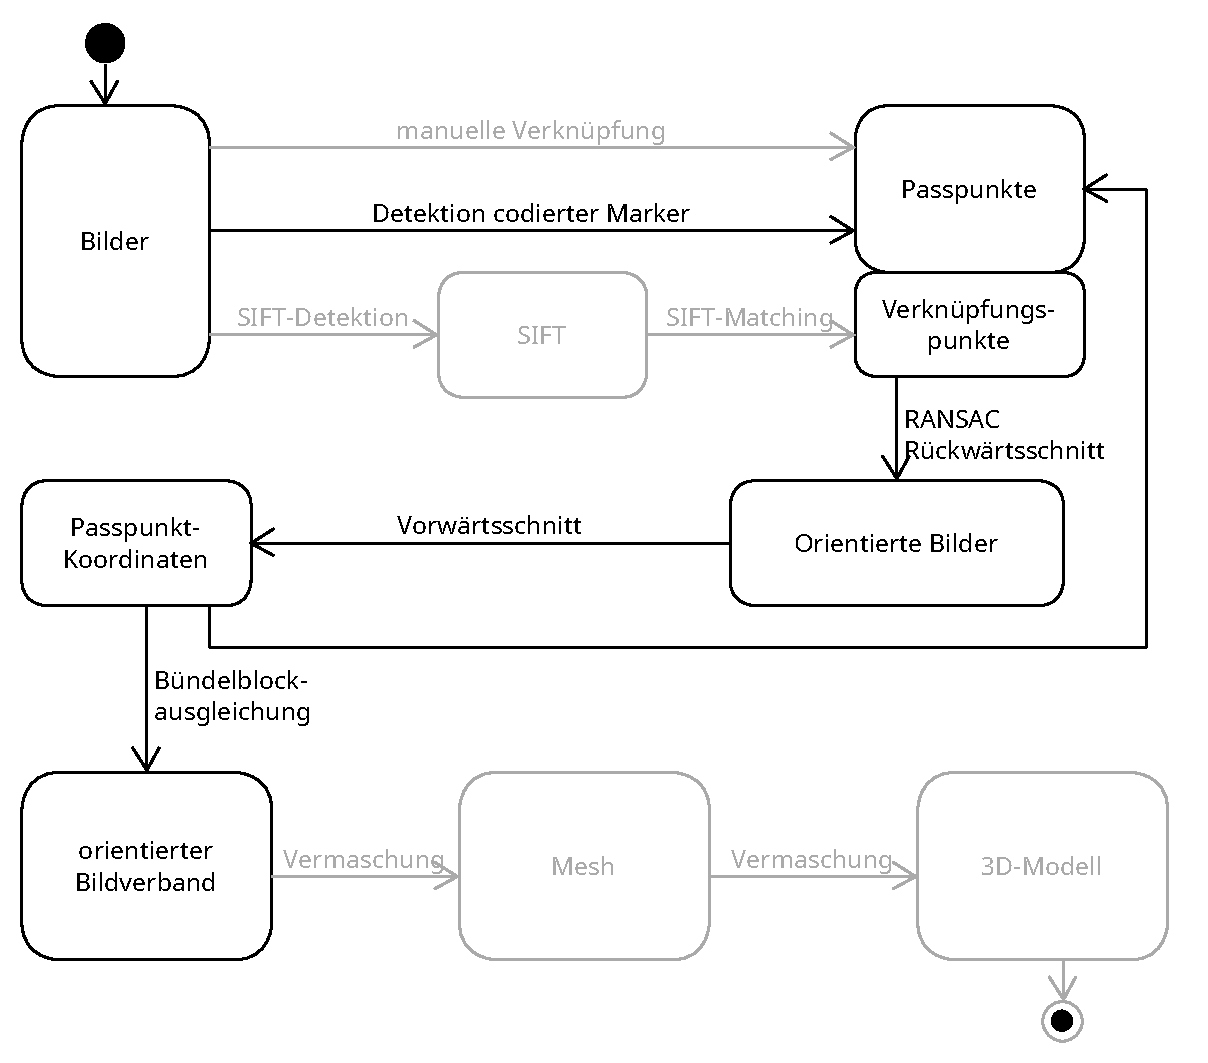
\includegraphics[width=0.8\textwidth]{./img/uml/uml_ablauf.pdf}
    \caption{Ablauf der Bildverknüpfung, nach \citealt[S. 492]{luhmann}} %Bildunterschrift
    \label{img:ablauf} %ID fürs Bild
\end{figure}


\section{Bilder}
\label{s:bilder}

Die Berechnung der Tiefeninformationen ist nur möglich, sofern der Punkt in mindestens einem weiteren Bild abgebildet ist. Die Genauigkeit der Berechnung ist vom Schnittwinkel dieser beiden Strahlen abhängig. Um möglichst gute Grundlagen zur Ver\-fügung zu haben und die innere und äußere Orientierung möglichst gut berechnen zu können, müssen diese Bilder einige Bedingungen erfüllen - auf diese wird in diesem Abschnitt eingegangen.

\subsection{Überlappung und Bildinhalte}
Da die Bilder durch identische Punkte verbunden werden, müssen die Bildinhalte sich überlappen und gemeinsame Punkte in den Bildern identifiziert werden. Die automatische Detektion von identischen Punkten ist auf verschiedene Weisen möglich: Entweder durch die Nutzung von uncodierten und codierten Passpunkten aber über eine Merkmalsextraktion. Für das letztere muss die Oberfläche aber genügend Textur bzw. Struktur aufweisen. Detailliert wird in \autoref{s:verknuepfung} hierauf eingegangen. \citep[S. 478]{luhmann}

\subsection{Position und Ausrichtung der Kamera}
Damit die Schnitte der Bildstrahlen optimal sind und die Berechnung der Tiefeninformationen möglichst genau ist, müssen die Kameras möglichst gleichmäßig um das Objekt verteilt sein.
Bilder, die vom gleichen Standpunkt aufgenommen wurden, sind oft nur ungenau verknüpfbar. Daher empfiehlt es sich, Bilder aus verschiedensten Richtungen zu machen, also bei der manuellen Photographie um das Objekt herumzugehen - eine Mehrbildaufnahme im Rundum-Verband zu erzeugen. \citep[S. 170]{luhmann}

Entsprechend müssen die Kameras an den Trägern auch gleichmäßig um das Objekt verteilt positioniert werden und dabei auch an die Form des Objektes wie Einschnitte anpassbar sein.

\subsection{Belichtung}
Um identische Punkte in den Bildern identifizieren zu können, müssen die Bilder eine gleichmäßige Beleuchtung aufweisen. Hierfür sollte es vermieden werden, dass Schatten auf das Objekt fallen. Eine gleichmäßige Beleuchtung kann durch die Nutzung von mehreren Lichtquellen erreicht werden. Auch sollte keine Blendwirkung entstehen, die durch direkte Sonneneinstrahlung oder Reflexionen entstehen kann. Die Belichtung der einzelnen Bilder sollte möglichst identisch sein, damit später auch eine zusammenhängende Texturierung möglich ist.
Da die Objekte und die Kameras sich während der Aufnahme nicht bewegen, kann die Belichtungszeit verlängert werden, um Rauschen durch eine zu hohe Sensorempfindlichkeit zu vermeiden und so die Bildqualität zu erhöhen.

\subsection{Innere Orientierung}
\label{s:innereorientierung}
Aus der Position eines Punktes in einem Bild kann, ähnlich einer Messung mit einem Theodolit, die Richtung des Punktes in Relation zu der Kamera bestimmt werden. Damit diese Berechnung möglich wird, müssen die Parameter der Kamera bekannt sein, die sogenannte innere Orientierung. Sie beschreibt die Abbildung der Kamera mathematisch. Wichtigste Parameter sind hierbei die Lage des Bildhauptpunktes und die Kamerakonstante. Außerdem zählen hierzu auch die Parameter, die die Verzeichnung beschreiben. \citep[S. 179f]{luhmann}

Jede Einstellung der Kameraoptik verändert die innere Orientierung und auch jede Kamera, auch einer Modellreihe, kann je nach Genauigkeitsanspruch als unterschiedlich angesehen werden. Änderungen können sich beispielsweise durch Umfokussierung oder die Nutzung eines optischen Zoom ergeben, aber auch durch einen mechanisch instabilen Aufbau der Kameras. Daher sollten die Bilder normalerweise möglichst mit nur einer Kamera mit festen Einstellungen (Brennweite, Fokus, Blende, Objektiv) aufgenommen werden. Änderungen der Empfindlichkeit (ISO-Zahl) oder Belichtungszeit sind unproblematisch für die innere Orientierung, da hierbei die Abbildungseigenschaften der Kamera nicht verändert werden. \citep[S. 176]{luhmann}

Die Bestimmung der inneren Orientierung, auch Kalibrierung genannt, kann während der Messung beispielsweise als Parameter in der Bündel\-block\-ausgleichung erfolgen. Je nach Stabilität der inneren Orientierung sind hier verschiedene Methoden möglich - beispielsweise die Kalibrierung jedes einzelnen Bildes bei instabilen Kameras, wie sie in diesem Projekt verwendet werden. \citep[S. 181f]{luhmann}

\subsection{Fokussierung und Schärfentiefe}
Um genaue Punktwolken zu ermöglichen, muss das Objekt scharf abgebildet werden. Die Kameras müssen dafür entsprechend fokussiert sein. Jedoch wird durch die Fokussierung auch die Innere Orientierung verändert. Normalerweise wird daher auf eine Umfokussierung verzichtet und mittels der Blende (kleine Blendenöffnung) die Schärfentiefe erhöht, sodass ein großer Bereich scharf abgebildet wird. Die Schärfentiefe ist jedoch im Makrobereich relativ klein. Genauer wird auf die Schärfentiefe in \autoref{sec:fokusstacking} eingegangen.


\section{Verknüpfungspunkte}
\label{s:verknuepfung}
Um die einzelnen Bilder verknüpfen zu können, werden identische Punkte zwischen zwei oder mehr Bildern benötigt. Diese können klassisch per Hand erfasst werden, jedoch ist dieses schon bei kleineren Projekten sehr zeitaufwändig. Daher wird meist die Möglichkeit genutzt, automatisch Verknüpfungspunkte zu erzeugen. Hierfür gibt es verschiedene Methoden, die im Folgenden vorgestellt werden.

\subsection{Zielmarker}
Es gibt verschiedenste Formen von Markern, die automatisch erfasst werden können. Grob unterschieden werden kann in codierte und nicht codierte Zielmarker. Beispiele für nicht codierte sind beispielsweise einfache kreisförmige Klebepunkte oder Marker, die aus Linien bestehen und ihren Mittelpunkt durch dessen Schnitt definieren.
Vorteilhaft ist jedoch die Verwendung von codierten Zielmarken. Hier können die Punkte direkt zugeordnet werden und es ist keine weitere Filterung und Berechnung zur Zuordnung notwendig. \citep[S.535ff]{luhmann}

\subsubsection{Zielmarken nach Schneider}
Beispielsweise von Agisoft Metashape werden Marker nach Schneider verwendet \citep{ccct}. Diese bestehen aus mehreren konzentrischen Kreisen und werden entsprechend auch als CCCT -- concentric circular coded target -- bezeichnet. Die Mitte des Markers wird durch den gemeinsamen Mittelpunkt der Kreise definiert.  Vorteilhaft ist, dass die Marker auch bei unscharfen Bildern erkannt werden können und ihr Zentrum auch manuell identifiziert werden kann. Sie haben sich daher als Standardmarker in der Photogrammetrie etabliert.\todo{Quelle}


\subsubsection{ArUco-Marker}
Eine andere Variante der automatischen Verknüpfungspunkte sind die sogenannten ArUco-Marker. Diese werden häufig für die Orientierung bei Augmented-Reality-Anwend\-ungen genutzt. Sie werden als codierte Messmarken verwendet und können automatisch im Subpixelbereich erkannt werden. Jede Ecke kann hier einzeln identifiziert werden, sodass ein erkannter Marker vier Verknüpfungspunkte liefern kann. Nachteilig ist, dass die Ecken nicht eindeutig identifiziert werden können, wenn die Aufnahme unscharf ist. Durch ihre Verwendung in der Informatik sind viele Bibliotheken für die Erkennung verfügbar, beispielsweise kann OpenCV diese identifizieren. %\citep[S. 536]{luhmann}


\subsection{Merkmalsextraktion}
Ohne das Anbringen von Markern können auch Merkmale in den Bildern erkannt werden. Hierfür gibt es verschiedene Methoden, eine dieser ist die SIFT-Methode, welche hier beispielhaft kurz dargestellt wird. Sie liefert Verknüpfungspunkte aus Mustern auf den photographierten Oberflächen. Es ist meist nicht notwendig explizit Marker an dem aufzunehmenden Objekt anzubringen, sofern seine Oberfläche nicht strukturlos ist (glatte weiße Wände etc.) oder in Bewegung ist.

Zur Erkennung von Merkmalen setzt das Verfahren auf die Detektion von Kanten. Diese werden in verschiedenen Stufen einer Bildpyramide erkannt und ihre Extrema berechnet. Es werden diese Merkmale weiter ausgedünnt, beispielsweise über den Kontrast. Sofern ein möglicher Marker identifiziert wurde, wird eine Beschreibung erzeugt. Diese erfolgt  durch Analyse der Helligkeitsabweichungen zu den Nachbar-Pixeln und wird an der stärksten Abweichung ausgerichtet. Hierdurch wird die Beschreibung dann richtungsunabhängig. Mit diesen kann dann die Übereinstimmung von zwei Markern in zwei Photos bestimmt werden, auch wenn die Bilder zueinander gekippt oder gedreht sind.
\citep[S. 484f]{luhmann}

\section{Verknüpfung von Bildern}
\label{s:photogramm}
Durch die beschriebenen Verfahren und die hieraus entstandenen Verknüpfungs\-punkte können die Bilder miteinander verknüpft werden. Da die Kamerapositionen am Rahmen veränderlich sind und die Montage auch keine ausreichend genaue Fixierung garantiert, können die bekannten Positionen aus vorherigen Messungen nur als Näherungswerte genutzt werden. Die genaue Bestimmung der Position und Ausrichtung - die äußere Orientierung - erfolgt dann über ein photogrammetrisches Verfahren. Dieses wird im Folgenden vorgestellt.


\subsection{Abbildung}
\todo{Abbildung allgemein erklären}
\label{ss:abbildungsgleichung}

\paragraph{Abbildungsgleichung}

Die Abbildung eines Punktes auf einem Bild wird durch die Abbildungsgleichung beschrieben. In der Matrizenrechnung ergibt sich dieser aus der Multiplikation mit der Projektionsmatrix $P$. Diese ergibt sich aus der Kameramatrix $K$, der Rotation $R$ und dem Projektionszentrum $X_0$. (siehe \autoref{abbildungsgleichung}, nach \citealp[S. 244]{hartley} und \citealp[S. 290]{luhmann})

\begin{align}
    \label{abbildungsgleichung}
    x' & = P \cdot X       \\
    P  & = K \cdot [R|X_0] \\
    P  & =
    \begin{bmatrix}
        c_x & 0   & x'_0 \\
        0   & c_y & y'_0 \\
        0   & 0   & 1
    \end{bmatrix}
    \cdot
    \begin{bmatrix}
        r_11 & r_21 & r_31 & X_0 \\
        r_12 & r_22 & r_32 & Y_0 \\
        r_13 & r_23 & r_33 & Z_0 \\
    \end{bmatrix}
\end{align}

Um die Beziehung zwischen zwei Bildern aufzustellen, kann man diese Abbildungsgleichung nutzen. Da es hier nur um die Beziehung zwischen zwei Bildern geht, kann die Rotation und Translation des ersten Bildes auf 0 gesetzt werden ($R$ ist dann eine 3x3-Einheitsmatrix und $X_0$ ein Nullvektor). $X_0$ des zweiten Bildes wird zur Translation zwischen den beiden Bildern. \citep[S. 330]{luhmann}
\todo{Überarbeiten und Verzeichnung hinzufügen}


\subsection{Rückwärtsschnitt}
Sofern Koordinaten von Passpunkten bekannt sind, können die Positionen und Ausrichtungen der Kameras berechnet werden. Hierfür wird der sogenannte Rückwärtsschnitt genutzt. Die Berechnung erfolgt auf Basis der Abbildungsgleichung, die die Position eines Punktes in einem Bild in Beziehung zur Kamera setzt. Für die Berechnung selbst gibt es verschiedene Methoden. Verwendet wurde hier der von OpenCV genutzte Ansatz von \citeauthor{Lepetit2008} in Kombination mit einem RANSAC-Ansatz. Durch die Nutzung des RANSAC-Ansatzes können veränderte Passpunkte identifiziert und als Ausreißer markiert werden.

\subsection{Vorwärtsschnitt}
Um wiederum aus einem Stereopaar mit bekannter innerer und äußerer Orientierung Punktkoordinaten zu berechnen, wird der Vorwärtsschnitt genutzt. Hierfür sind die Bildkoordinaten des zu berechnenden Punktes in beiden Bildern notwendig.

Mit dem Vorwärts\-schnitt können neben markierten Verknüpfungspunkten auch die Neupunkte, die mittels SIFT oder ähnlichen Bild\-erkennungs\-algorithmen erkannt wurden, berechnet werden. Dadurch kann eine dünne Punktwolke erzeugt werden, die dann in der Bündel\-block\-ausgleichung weiter optimiert werden kann.

\begin{comment}
Die Koordinaten der Passpunkt-Ausreißer aus der Berechnung der Kamerapositionen werden anschließend neu berechnet. Hierfür wird der Vorwärtsschnitt genutzt. Auch hier wird OpenCV zur Berechnung genutzt. Die Berechnung der Passpunkte erfolgt für jedes Bildpaar einzeln. Für alle Koordinaten wird dann pro Passpunkt der Z-Score berechnet. Passpunkte, die einen Z-Score von über 2 haben, werden als Ausreißer markiert und nicht weiter betrachtet.
\end{comment}

\section{Bündelblockausgleichung}
\label{s:buendelblock}
Mittels Bündelblockausgleichung können die grob mit den vorher genannten Verfahren bestimmten Positionen und Drehungen in einer Ausgleichung optimiert werden. Hierzu gehen alle Parameter der Bilder und die Positionen der Passpunkte in die gemeinsame Ausgleichung ein. Grundlage der Ausgleichung ist die in \autoref{ss:abbildungsgleichung} beschriebene Abbildungsgleichung. Als Ergebnis erhält man die ausgeglichenen Parameter und Genauigkeitsangaben für diese. \citep[S. 343ff]{luhmann}


\section{Multi-view Stereo}
\todo{überprüfen, falsch?}
Die dünne Punktwolke aus dem Vorwärtsschnitt kann durch Multi-view Stereo-Verfahren zu einem 3D-Modell erweitert werden. Hierbei werden jeweils Bildpaare gebildet und die Disparitäten, also die Verschiebung des Objektes in der Abbildung, bestimmt. Diese sind abhängig von der Entfernung des Objektes, bei einem unendlich weit entfernten Objekt tritt keine Disparität auf \citep[S. 313]{luhmann}. Die Disparitäten können dann in Tiefeninformationen umgerechnet werden. Diese können dann wiederum gemittelt und zu einen Tiefenbild zusammengefasst werden. \citep[S. 505]{luhmann}
%\citep[S. 51]{opendronemap}

\section{Mesh-Generierung}
Bis zu diesem Schritt besteht das Modell nur aus einzelnen Punkten, die keine Oberfläche ergeben. Um ein 3D-Modell zu erhalten, muss eine Oberfläche generiert werden. Hierfür wird ein Mesh-Generierungsverfahren genutzt. Hierbei wird die Punktwolke in Dreiecke unterteilt. Hierfür gibt es verschiedene Verfahren, die sich in der Art der Unterteilung unterscheiden. OpenDroneMap nutzt beispielsweise die Screened Poisson Surface Reconstruction. \citep[S. 52f]{opendronemap}

Die Screened Poisson Surface Reconstruction ist ein Verfahren, das auf der Poisson-Gleichung basiert. Diese wird genutzt, um die Oberfläche zu glätten und zu interpolieren. Ein Teil des Ansatzes ist es, dass die Ausrichtung der Punkte berücksichtigt wird. Die Punkte werden hierbei in eine Gitterstruktur überführt und die Oberfläche durch die Lösung der Poisson-Gleichung bestimmt. \citep{spsr}
\todo{Details zur Poisson-Gleichung}

\section{Texturierung}
Abschließend wird das Modell texturiert. Hierfür werden die Bilder, die zur Erstellung des Modells genutzt wurden, auf das Modell projiziert. Außerdem werden Helligkeits- und Farbunterschiede ausgeglichenen. \citep[S. 54f]{opendronemap}
\todo{erweitern}

\biblio
\end{document}